\documentclass{minimal}
\usepackage{epsfig,color}
\usepackage{units}
\usepackage[papersize={576.00bp,432.00bp},text={576.00bp,432.00bp}]{geometry}
\begin{document}
\centering
% Title: glps_renderer figure
% Creator: GL2PS 1.3.8, (C) 1999-2012 C. Geuzaine
% For: Octave
% CreationDate: Wed Oct 29 20:10:09 2014
\setlength{\unitlength}{1pt}
\begin{picture}(0,0)
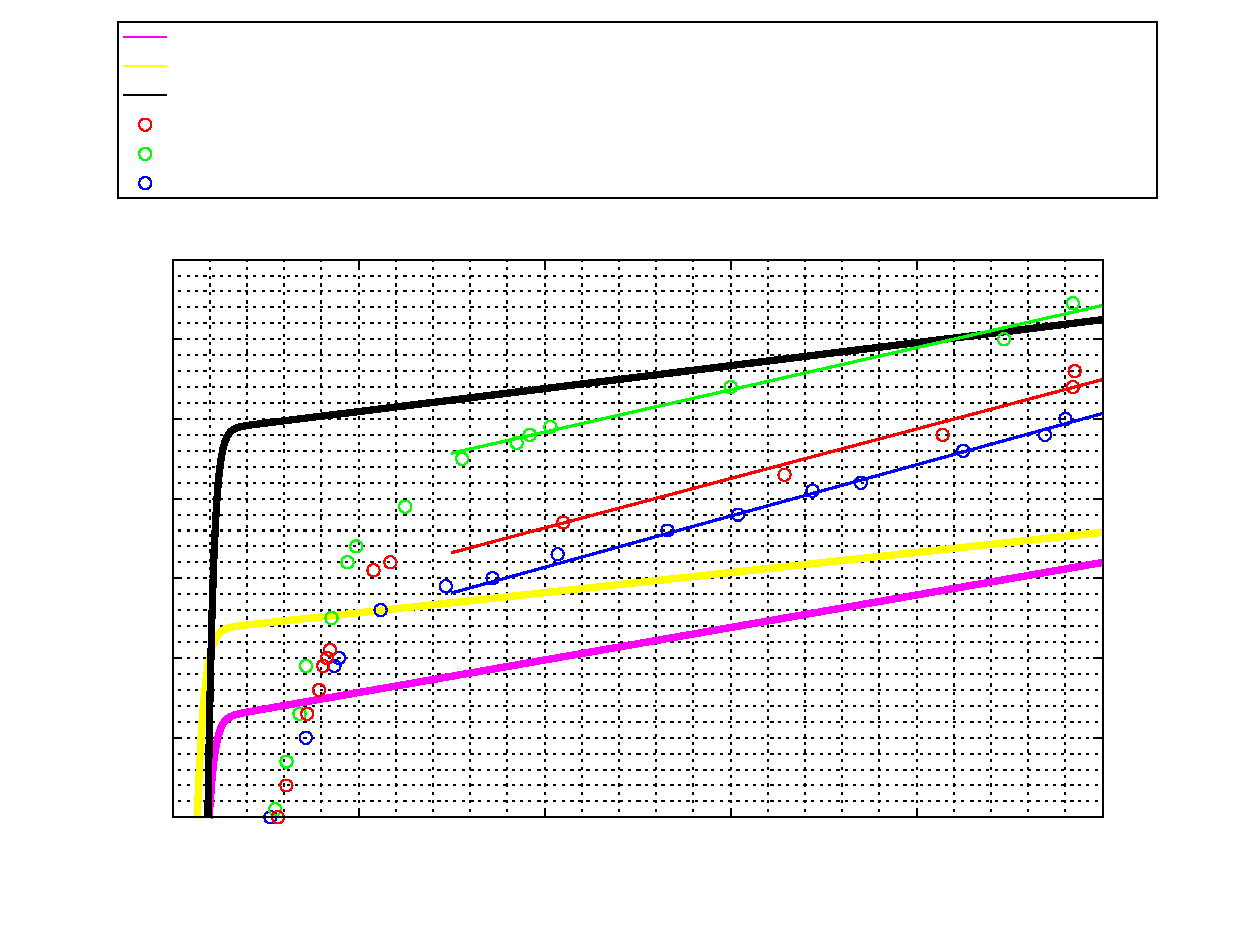
\includegraphics{IcvsVce_25mA-inc}
\end{picture}%
\begin{picture}(576,432)(0,0)
\fontsize{10}{0}
\selectfont\put(74.88,42.5253){\makebox(0,0)[t]{\textcolor[rgb]{0,0,0}{{0}}}}
\fontsize{10}{0}
\selectfont\put(164.16,42.5253){\makebox(0,0)[t]{\textcolor[rgb]{0,0,0}{{1000}}}}
\fontsize{10}{0}
\selectfont\put(253.44,42.5253){\makebox(0,0)[t]{\textcolor[rgb]{0,0,0}{{2000}}}}
\fontsize{10}{0}
\selectfont\put(342.72,42.5253){\makebox(0,0)[t]{\textcolor[rgb]{0,0,0}{{3000}}}}
\fontsize{10}{0}
\selectfont\put(432,42.5253){\makebox(0,0)[t]{\textcolor[rgb]{0,0,0}{{4000}}}}
\fontsize{10}{0}
\selectfont\put(521.28,42.5253){\makebox(0,0)[t]{\textcolor[rgb]{0,0,0}{{5000}}}}
\fontsize{10}{0}
\selectfont\put(69.8755,47.52){\makebox(0,0)[r]{\textcolor[rgb]{0,0,0}{{20}}}}
\fontsize{10}{0}
\selectfont\put(69.8755,85.7657){\makebox(0,0)[r]{\textcolor[rgb]{0,0,0}{{21}}}}
\fontsize{10}{0}
\selectfont\put(69.8755,124.011){\makebox(0,0)[r]{\textcolor[rgb]{0,0,0}{{22}}}}
\fontsize{10}{0}
\selectfont\put(69.8755,162.257){\makebox(0,0)[r]{\textcolor[rgb]{0,0,0}{{23}}}}
\fontsize{10}{0}
\selectfont\put(69.8755,200.503){\makebox(0,0)[r]{\textcolor[rgb]{0,0,0}{{24}}}}
\fontsize{10}{0}
\selectfont\put(69.8755,238.748){\makebox(0,0)[r]{\textcolor[rgb]{0,0,0}{{25}}}}
\fontsize{10}{0}
\selectfont\put(69.8755,276.994){\makebox(0,0)[r]{\textcolor[rgb]{0,0,0}{{26}}}}
\fontsize{10}{0}
\selectfont\put(69.8755,315.239){\makebox(0,0)[r]{\textcolor[rgb]{0,0,0}{{27}}}}
\fontsize{10}{0}
\selectfont\put(298.08,31.5253){\makebox(0,0)[t]{\textcolor[rgb]{0,0,0}{{$V_{CE} [\unit{mV}]$}}}}
\fontsize{10}{0}
\selectfont\put(53.8755,181.38){\rotatebox{90}{\makebox(0,0)[b]{\textcolor[rgb]{0,0,0}{{$I_C [\unit{mA}]$}}}}}
\fontsize{10}{0}
\selectfont\put(74.7211,422.224){\makebox(0,0)[l]{\textcolor[rgb]{0,0,0}{{\texttt{PHIL\_BJT} $r_o = 2,450199\unit{k\Omega}$  $V_A= 51,84079\unit{V}$ $I_{C_{sat}} = 21,157789 \unit{mA}$}}}}
\fontsize{10}{0}
\selectfont\put(74.7211,408.164){\makebox(0,0)[l]{\textcolor[rgb]{0,0,0}{{\texttt{SIEMENS} $r_o = 3,960928\unit{k\Omega}$  $V_A= 88,38723\unit{V}$ $I_{C_{sat}} = 22,314781 \unit{mA}$}}}}
\fontsize{10}{0}
\selectfont\put(74.7211,394.104){\makebox(0,0)[l]{\textcolor[rgb]{0,0,0}{{modelo modificado $r_o = 3,462771\unit{k\Omega}$  $V_A= 98,24354\unit{V}$ $I_{C_{sat}} = 24,803164 \unit{mA}$}}}}
\fontsize{10}{0}
\selectfont\put(74.7211,380.044){\makebox(0,0)[l]{\textcolor[rgb]{0,0,0}{{transistor 1 $r_o = 1,610301\unit{k\Omega}$  $V_A= 36,05432\unit{V}$ $I_{C_{sat}} = 22,389798 \unit{mA}$}}}}
\fontsize{10}{0}
\selectfont\put(74.7211,365.984){\makebox(0,0)[l]{\textcolor[rgb]{0,0,0}{{transistor 2 $r_o = 1,886962\unit{k\Omega}$  $V_A= 33,94572\unit{V}$ $I_{C_{sat}} = 23,775390 \unit{mA}$}}}}
\fontsize{10}{0}
\selectfont\put(74.7211,351.924){\makebox(0,0)[l]{\textcolor[rgb]{0,0,0}{{transistor 3 $r_o = 1,553545\unit{k\Omega}$  $V_A= 44,86326\unit{V}$ $I_{C_{sat}} = 21,850496 \unit{mA}$}}}}
\end{picture}
\end{document}
